\documentclass{article}

\usepackage{tikz}
\usepackage{aeguill}
\usepackage{csquotes}
\usepackage{blindtext}

\begin{document}

\title{Usefulness of SSM and UML in Designing a Web Syndication System for the World Service}
\author{James Donohue}

\maketitle

\begin{abstract}
A collection of thoughts and ideas about random disconnected things.
\end{abstract}

\section{Introduction}
\subsection{Background}

The BBC World Service website portfolio, which currently includes 27 sites but will soon increase to nearly 40, offers news to millions of users around the world in their own language. A publicly-stated ambition of the BBC is to increase its global audience to 500 million by 2022 (British Broadcasting Corporation (BBC) 2013). One way it can contribute to this effort is through web syndication.

Web syndication allows website owners to publish information about new or changed content in a way that can be reused by other websites or end users. Standards for web syndication have existed in some form since 1997 (World Wide Web Consortium (W3C) 1997), the dominant formats today being RSS (Really Simple Syndication) and Atom (both of these are XML-based and offer a similar feature set; for the purpose of this study they are treated as interchangeable).

At the time of writing the World Service sites are being migrated to a new content management system (CMS) and the 'Public Feeds Adaptor' that formerly generated Atom feeds for these sites is going to be decommissioned. Therefore a new system based around the new CMS must be implemented in order to maintain web syndication capability for the existing 27 sites, and to ensure that it is available for the new ones that will be added.

\subsection{Aims of this study}

This study will examine how Soft Systems Methodology (SSM) and the Unified Modeling Language (UML) might be used in the design of a replacement system for web syndication, and to evaluate the usefulness of these approaches for the current problem. For the purposes of this study, it is assumed that a new 'ideal' system will be built that entirely replaces, and if possible improves upon, the previous one. However, other options are available, such as adapting the legacy system to interoperate with the new CMS. One reason for this assumption is to allow the author freedom to use full range of UML techniques without being constrained by the existing architecture.

The UML artefacts generated during the investigation will be used as a partial design for the new system which is to be built. It is hoped that once the system is operational there will be further opportunities to reflect on the relevance of the modelling techniques used by comparing this study with the finished product. In addition, it is the author's aim that the results of this investigation, along with the areas for further research and analysis suggested in the final section, will provide insights as to how organisations such as the BBC could make use of these modelling techniques in future projects.

\subsection{Contextualising the Problem}

In the terminology of Soft Systems Methodology (SSM), the starting point is a perceived 'problematical situation' which is made the subject of a series of learning-focused activities. Checkland and Poulter (2006) see SSM as a shift from the supposed 'positivism' of 1950s and 1960s methods which saught to solve real-world problems objectively to a phenomenological approach in which the the \textit{Weltanschauung}, or worldview, of all actors is emphasised.

The first Soft Systems activity centres around finding out about the problematic situation. To do this, a \textit{rich picture} may be created as an aide to exploring the context of the problem, and particularly to capture the "rich moving pageant of relationships" (Checkland and Scholes 1990, p.45) between the entities involved. Figure~\ref{rich-picture} shows such a rich picture for the present problem. 

\begin{figure}
  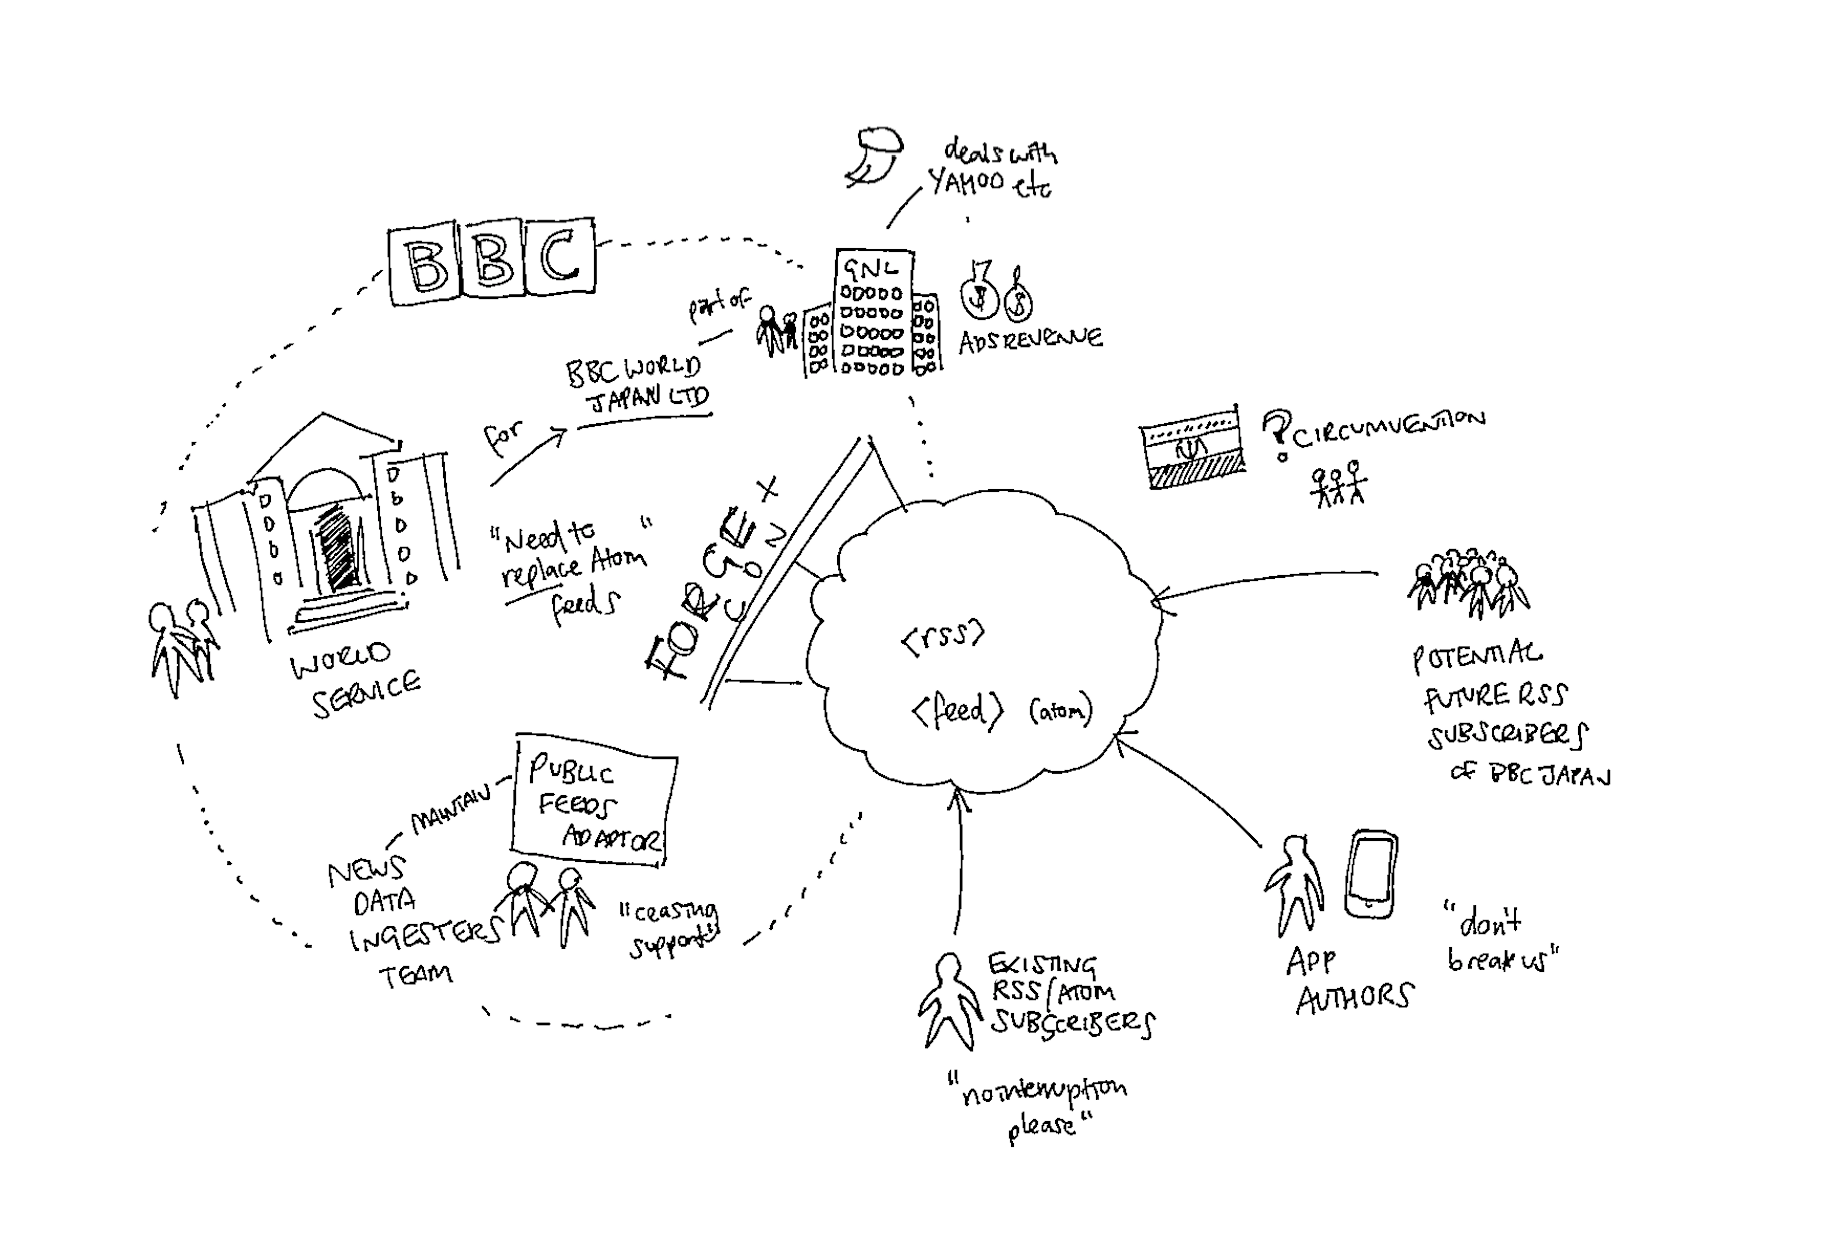
\includegraphics[width=\textwidth]{richpicture.png}
  \caption{Rich Picture of the BBC's problematic situation}
  \label{rich-picture}
\end{figure}

Our rich picture suggests some of the actors whose worldview we should consider. Indeed, SSM's role analysis (known as 'Analysis One') expands the definition of 'issue owner' to be anyone who may be "concerned about or affected by the situation and the outcome" (Checkland and Poulter 2006, p.28). From this perspective, the owners of the issue include the News Product Development Group, the BBC Trust, the Public Feeds Adaptor team and the World Service editorial staff, but members of the public currently subscribed to feeds, builders of third-party apps that consume the feeds, and even potential future users who do not currently use the feeds.

Next, SSM proposes the creation of a number of models showing 'purposeful activity' within a worldview that is made explicit. The starting point for each model is a root definition that describes the system as a statement using the PQR formula (Checkland and Poulter 2006, p.39). Taking one example from the rich picture, we can write the following root definition:

\begin{displayquote}
A system to provide a new web syndication platform for World Service sites by automatically generating and serving up-to-date RSS feeds, in order to allow users to receive updates about new and changed content and therefore contribute to an increase in traffic.
\end{displayquote}

As a further step to enrich our understanding of this system, Soft Systems encourages us to consider the mnemonic CATWOE (Checkland and Poulter 2006, p.42). Through this we might see a transformation (the T) from a deprecated legacy system with no support for the new CMS, to a better-supported and more flexible platform that will meet the BBC's wider needs in years to come. CATWOE offers a distinction between actors (who are involved in the system's activities), owners and customers who are affected by it. This allows us to refine our list of users given earlier.

Finally, we should give consideration to environment (the E of CATWOE). There are several dimensions to this, including the operational environment of the BBC itself, but also the context of the changing landscape of web syndication in the age of Twitter and Facebook. These considerations, and what impact they have on the actors involved, will be reflected in the use case diagrams and other artefacts produced in the next section.

% What about a diagram of an actual SSM purposeful system?
% Add project glossary?

% Stefano did 'Problem space contextualisation' and then 'Design'
% Ross did 'The problem' with 'Design goals' before moving on to Soft Systems

% Hoseyin suggested sections: 'literature review', 'methodology' and 'results'
% See notes from day

\subsection{Project glossary}

\begin{description}

\item [Syndication feed]
A feed of syndication stuff

\item [Subscriber]
blah

\end{description}

\section{Results}

In this section we present a series of UML diagrams that explore the problem domain described above. These diagrams are organised according to some of the workflows within the software development lifecycle defined by the Unified Process (UP) [ref?].

\subsection{Requirements}

From the root definition and list of actors given earlier, we can create the UML use case diagram shown in Figure~\ref{use-cases} which is non-comprehensive depiction of some of the use cases that the system must support. For the purposes of this diagram three actors have been identified, which represent three roles that users of the system may occupy. Further roles could be added in response to later analysis, since as Arlow and Neustadt (2005, p.74) stress, use case modelling is an iterative process. This provisionality applies equally to the system boundary (represented by the black rectangle) that indicates the \textit{subject} of the diagram.

\begin{figure}
  \includegraphics[width=\textwidth]{usecases.png}
  \caption{A use case diagram}
  \label{use-cases}
\end{figure}

In order to describe each use case in more detail, we can use the tabular structure for use case specifications recommended by Arlow and Neustadt (2005), an example of which for one of the use cases shown in Figure~\ref{use-cases} (\texttt{GetFeed}), can be seen in Table~\ref{use-case-detail}. In this use case the primary actor (the one who triggers the use case) is the \texttt{Subscriber}. This use case has one major possible alternative flow, which occurs when the subscriber requests a non-existent feed and is shown in Table~\ref{use-case-alt-detail}. An alternative approach would have been to use the \textit{If} and \textit{Else} keywords within the main flow of Table~\ref{use-case-detail} to describe an alternate flow without creating an entire separate specification. This option was rejected on the grounds that it might hinder intelligibility for non-technical readers, since "use cases are all about communication with the stakeholders" (Arlow and Neustadt 2005, p.101).

% More discussion of stakeholder difficulties with advanced use case features point on p110
% TODO discuss merits of using <<include>> etc. and why we reject it?

\begin{table}[]
\begin{center}
\begin{tabular}{ | p{\textwidth} |}
\hline
\multicolumn{1}{|c|}{Use case: GetFeed} \\
\hline
ID: 1 \\
\hline
Brief description: \\
The system return a web syndication feed containing information about content that has recently been created or updated \\
\hline
Primary actors: \\
Subscriber \\
\hline
Secondary actors: \\
None \\
\hline
Preconditions: \\
None \\
\hline
Main flow: \\
1. The use case starts when the Subscriber requests a feed via the network \\
2. The system verifies that there is content for the feed \\
3. The system generates the feed using the options given in the request \\
4. The system returns the generated feed to the Subscriber \\
\hline
Postconditions: \\
None \\
\hline
Alternative flows: \\
GetFeed:MissingFeed \\
\hline
\end{tabular}
\end{center}
\caption{Example of a use case specification}
\label{use-case-detail}
\end{table}

\begin{table}[]
\begin{center}
\begin{tabular}{ | p{\textwidth} |}
\hline
\multicolumn{1}{|c|}{Alternative flow: GetFeed:MissingFeed} \\
\hline
ID: 1.1 \\
\hline
Brief description: \\
The system notifies the user that the requested feed does not exist. \\
\hline
Primary actors: \\
Subscriber \\
\hline
Secondary actors: \\
None \\
\hline
Preconditions: \\
1. There is no content for the requested feed. \\
\hline
Alternative flow: \\
1. The alternative flow begings after step 2 of the main flow. \\
2. The system displays an error message to the Subscriber \\
\hline
Postconditions: \\
None \\
\hline
\end{tabular}
\end{center}
\caption{Example of a use case alternative flow specification}
\label{use-case-alt-detail}
\end{table}

\subsection{Analysis}

The use cases identified in the previous section can be used to produce an analysis model that focuses on \textit{what} the system does (but not yet \textit{how} it does it). Any artefacts produced in this workflow should remain useful to as many stakeholders as possible by using language from the business domain and avoiding implementation details (Arlow and Neustadt 2005, p.122).

The subject of the present study suggests the analysis classes shown in Figure~\ref{analysis-classes}. The classes were identified using noun/verb analysis of the project glossary and use cases above, and named based on clearly identifiable 'real world' concepts within the problem domain. They are necessarily high-level at this stage; moreover, features that are typically considerations of design rather than analysis, such as operation parameters, visibility adornments and constructors, have been omitted (Arlow and Neustadt 2005, p137-8, p148). The only operations represented (\texttt{addItem()} and \texttt{removeItem()}) are those that may give rise to a state transitions. Note that the \texttt{items} attribute of the \texttt{Feed} class is shown with the multiplicity expression \texttt{[0..*]} to indicate that \texttt{null} is a possible value for this attribute, if there are no items.

It should be noted that although the analysis model is intended to represent a generic syndication feed, irrespective of any specific serialisation format, it is somewhat aligned to the structure described by the RSS 2.0 Specification\ref{rss}. This is because ...

Also excluded from this diagram are 'getter' and 'setter' methods for each of the attributes. These could be represented as pairs of operations for each attribute, e.g. \texttt{getLanguage()} and \texttt{setLanguage()}. Ambler (2005, p.52) considers terms such operations "scaffolding code" and points out they are often be automatically generated by modelling tools. Excluding them from class diagrams may allow readers to more easily see the most significant operations.

As an alternative to representing class associations diagramatically, we could have shown these relationships using an explicit attribute within the class icon [?] (for example, \texttt{items : FeedItem[0..*]}). The diagramatic approach is in my view easier to immedaitely understand, and avoids having to make assumptions about how associations are implemented during analysis.

To indicate navigability between classes, I have followed Arlow and Neustadt (2005) in suppressing crosses and using a single arrow for unidirectional associations. Following this idiom, it is implicit that the association between \texttt{Feed} and \texttt{Site}, for example, is bidirectional, whereas the association between \texttt{FeedItem} and \texttt{Image} is explicitly one-way. This improves the overall legibility of the diagram, at the expense of some ambiguity.

Although UML supports adding role names at one or both ends of an association to indicate how each class is involved, Ambler (2005, p.65) states that the association name should be sufficient to make roles clear, reserving explicit role names for situations where there are multiple associations between the same classes.


% TODO 
% add a generalization relationship to class diagram
% add object diagram
% "in analysis class diagrams, you only show the classes, attributes and operations that illustrate the point you are trying to make" (p.259)

% TODO
% discuss alternative models - cohesion? coupling? see p161 and ch.15
%   avoiding deep inheriteance p163
%   risks of overiding a concrete methid p215

\begin{figure}
  \begin{center}
    \includegraphics[width=\textwidth]{classes.png}
  \end{center}
  \label{analysis-classes}
  \caption{Analysis classes}
\end{figure}

\subsection{Use case realisation}

% Interaction diagrams
% - add logging?
% - Sequence diagram in analysis omits user interface and focuses only on analysis class interaction! p251
% - Choice whether to use activations and message returns or not (e.g. p253)
%   - activation line ambiguity, e.g. is Feed active?
% - Add state invariant and/or constraint?
% - use of notes
% - activity diagrams part of dynamic view of system - not static structure of classes

% Why no design? because agile?

Use case realisation allows us to investigate how analysis classes collaborate in order to bring about the behaviour specified by a use case (Arlow and Neustadt 2005, p. 241). UML sequence diagrams depict a time-ordered series of interations between instances of different classifiers (here, analysis classes). This allows us a dynamic view of some of the static class structure seen in the last section.

Figure~\ref{sequence-diagram} shows a sequence diagram which realises the 'GetFeed' use case seen earlier.

The result of the \texttt{validateFeed} self-delegation message sent by \texttt{FeedBroker} is assigned to a temporary variable, \texttt{isValid}. This enables it to be used in the guard conditions of the \texttt{alt} operator (is there an alternative?)

\subsection{Activity}

\subsection{Method}

The figures in this study were generated using PlantUML, a free open-source tool\cite{plantuml} that generates UML artefacts from plain text files.

The UML 2.0 Superstructure specification states that interaction diagrams (of which sequence diagrams are a specialised form) are surrounded by a "solid-outline rectangle" including the interaction name in the upper left corner (OMG 2011, p.496). Since at the time of writing \texttt{plantuml} does not support automatically generating this rectangle, it has been manually added before inclusion in this document. Interestingly, \texttt{plantuml} can produce a 'frame' icon that fits the above description when generating deployment diagrams. Since \texttt{plantuml} is open source software, a helpful contribution would be to add support for automatically adding the rectangle and title to interaction diagrams in order to make them compliant with the specification. 

Note that frames have not been added to the other diagram types such as class diagrams because they are not mandated by the specification for these types (OMG 2011, p.691). This follows the approach taken in the figures in Arlow and Neustadt (2005).

\begin{figure}
  \begin{center}
    \includegraphics[width=\textwidth]{sequence.png}
  \end{center}
  \label{sequence-diagram}
  \caption{Sequence diagram for 'GetFeed'}
\end{figure}

\clearpage

\section{Evaluation}

\subsection{Caching}

One technical constraint placed on the system is the technology stack to be used. In order to promote cooperation and resource sharing between different BBC divisions, Morph, a new Node.js application platform developed by BBC Sport, is being used to generate feeds.

Like most dynamic web applications [ref?], Morph uses a pull-based model for generating content, since the trigger for resource generation is a request by an HTTP user agent. Once generated, representations are cached (using Redis, and optionally, Amazon S3). What is different about Morph is that in the event of a cache miss, it immediately returns a \texttt{202 Accepted} HTTP response to the user, while the request to generate content is queued for asynchronous processing. 

This corresponds to the 'Fail Fast' design pattern proposed by Nygard (2007), in that the API responds immediately when it determines that it does not have any representation available. One benefit of this approach is that the client can implement a variety of different strategies for retrying and/or recovering, depending on the type of data or functionality being provided.

% Rich pictures are never finished, they should evolve as enquiry progresses (LFA p25)

% How diagrams were generated
% Limitations of tools (e.g. no package border around interaction diagrams)
% diagrams not done (e.g. y no communication diagrams?)

\section{Conclusion}
Nothing besides remains.

\begin{thebibliography}{9}

\bibitem{bbc2013} 
British Broadcasting Corporation (BBC), 2013.
\textit{BBC announces ambition to double global audience to 500 million} [online].
Available from: http://www.bbc.co.uk/mediacentre/latestnews/2013/dg-global-audience [Accessed 24 June 2016].

\bibitem{w3c1997} 
World Wide Web Consortium (W3C), 1997.
\textit{Channel Definition Format (CDF)} [online].
Available from: https://www.w3.org/TR/NOTE-CDFsubmit.html
[Accessed 24 July 2016].

\bibitem{checkland1990}
Checkland, P. and Scholes, J. 1990.
\textit{Soft Systems Methodology in Action}.
Chichester: John Wiley

\bibitem{checkland2006} 
Checkland, P. and Poulter, J., 2006.
\textit{Learning for Action: A Short Definitive Account of Soft Systems Methodology and its use for Practitioners, Teachers and Students}.
Chichester: John Wiley

\bibitem{arlow} 
Arlow, J. and Neustadt, I., 2005.
\textit{UML 2 and the Unified Process}. Second Edition.
Upper Saddle River, NJ: Addison-Wesley

\bibitem{ambler}
Ambler, S. W., 2005.
\textit{The Elements of UML 2.0 Style}.
New York, NY: Cambridge University Press

\bibitem{nygard}
Nygard, M. T., 2007.
\textit{Release It!: Design and Deploy Production-Ready Software}.
Raleigh, North Carolina: The Pragmatic Bookshelf

\bibitem{omg2011} 
Object Management Group (OMG), 2011.
\textit{OMG Unified Modeling Language (OMG UML), Superstructure}. Version 2.4.1 [online].
Available from: http://www.omg.org/spec/UML/2.4.1/Superstructure
[Accessed 14 August 2016].

\bibitem{plantuml}
PlantUML.com, 2016.
\textit{Frequently Asked Questions} [online].
Available from: http://plantuml.com/faq.html
[Accessed 14 August 2016].

\bibitem{rss}
RSS Advisory Board, 2009
\textit{RSS 2.0 Specification}. Version 2.0.11 [online].
Available from: http://www.rssboard.org/rss-specification
[Accessed 14 August 2016].

\bibitem{atomrss}
Ruby, S., 2008.
\textit{Rss20AndAtom10Compared} [online].
Available from: http://www.intertwingly.net/wiki/pie/Rss20AndAtom10Compared
[Accessed 14 August 2016].

\end{thebibliography}

\end{document}

